\documentclass[]{article}
\usepackage{lmodern}
\usepackage{amssymb,amsmath}
\usepackage{ifxetex,ifluatex}
\usepackage{fixltx2e} % provides \textsubscript
\ifnum 0\ifxetex 1\fi\ifluatex 1\fi=0 % if pdftex
  \usepackage[T1]{fontenc}
  \usepackage[utf8]{inputenc}
\else % if luatex or xelatex
  \ifxetex
    \usepackage{mathspec}
  \else
    \usepackage{fontspec}
  \fi
  \defaultfontfeatures{Ligatures=TeX,Scale=MatchLowercase}
\fi
% use upquote if available, for straight quotes in verbatim environments
\IfFileExists{upquote.sty}{\usepackage{upquote}}{}
% use microtype if available
\IfFileExists{microtype.sty}{%
\usepackage{microtype}
\UseMicrotypeSet[protrusion]{basicmath} % disable protrusion for tt fonts
}{}
\usepackage[margin=1in]{geometry}
\usepackage{hyperref}
\hypersetup{unicode=true,
            pdftitle={Atlas-PS 3},
            pdfauthor={David Atlas},
            pdfborder={0 0 0},
            breaklinks=true}
\urlstyle{same}  % don't use monospace font for urls
\usepackage{color}
\usepackage{fancyvrb}
\newcommand{\VerbBar}{|}
\newcommand{\VERB}{\Verb[commandchars=\\\{\}]}
\DefineVerbatimEnvironment{Highlighting}{Verbatim}{commandchars=\\\{\}}
% Add ',fontsize=\small' for more characters per line
\usepackage{framed}
\definecolor{shadecolor}{RGB}{248,248,248}
\newenvironment{Shaded}{\begin{snugshade}}{\end{snugshade}}
\newcommand{\KeywordTok}[1]{\textcolor[rgb]{0.13,0.29,0.53}{\textbf{{#1}}}}
\newcommand{\DataTypeTok}[1]{\textcolor[rgb]{0.13,0.29,0.53}{{#1}}}
\newcommand{\DecValTok}[1]{\textcolor[rgb]{0.00,0.00,0.81}{{#1}}}
\newcommand{\BaseNTok}[1]{\textcolor[rgb]{0.00,0.00,0.81}{{#1}}}
\newcommand{\FloatTok}[1]{\textcolor[rgb]{0.00,0.00,0.81}{{#1}}}
\newcommand{\ConstantTok}[1]{\textcolor[rgb]{0.00,0.00,0.00}{{#1}}}
\newcommand{\CharTok}[1]{\textcolor[rgb]{0.31,0.60,0.02}{{#1}}}
\newcommand{\SpecialCharTok}[1]{\textcolor[rgb]{0.00,0.00,0.00}{{#1}}}
\newcommand{\StringTok}[1]{\textcolor[rgb]{0.31,0.60,0.02}{{#1}}}
\newcommand{\VerbatimStringTok}[1]{\textcolor[rgb]{0.31,0.60,0.02}{{#1}}}
\newcommand{\SpecialStringTok}[1]{\textcolor[rgb]{0.31,0.60,0.02}{{#1}}}
\newcommand{\ImportTok}[1]{{#1}}
\newcommand{\CommentTok}[1]{\textcolor[rgb]{0.56,0.35,0.01}{\textit{{#1}}}}
\newcommand{\DocumentationTok}[1]{\textcolor[rgb]{0.56,0.35,0.01}{\textbf{\textit{{#1}}}}}
\newcommand{\AnnotationTok}[1]{\textcolor[rgb]{0.56,0.35,0.01}{\textbf{\textit{{#1}}}}}
\newcommand{\CommentVarTok}[1]{\textcolor[rgb]{0.56,0.35,0.01}{\textbf{\textit{{#1}}}}}
\newcommand{\OtherTok}[1]{\textcolor[rgb]{0.56,0.35,0.01}{{#1}}}
\newcommand{\FunctionTok}[1]{\textcolor[rgb]{0.00,0.00,0.00}{{#1}}}
\newcommand{\VariableTok}[1]{\textcolor[rgb]{0.00,0.00,0.00}{{#1}}}
\newcommand{\ControlFlowTok}[1]{\textcolor[rgb]{0.13,0.29,0.53}{\textbf{{#1}}}}
\newcommand{\OperatorTok}[1]{\textcolor[rgb]{0.81,0.36,0.00}{\textbf{{#1}}}}
\newcommand{\BuiltInTok}[1]{{#1}}
\newcommand{\ExtensionTok}[1]{{#1}}
\newcommand{\PreprocessorTok}[1]{\textcolor[rgb]{0.56,0.35,0.01}{\textit{{#1}}}}
\newcommand{\AttributeTok}[1]{\textcolor[rgb]{0.77,0.63,0.00}{{#1}}}
\newcommand{\RegionMarkerTok}[1]{{#1}}
\newcommand{\InformationTok}[1]{\textcolor[rgb]{0.56,0.35,0.01}{\textbf{\textit{{#1}}}}}
\newcommand{\WarningTok}[1]{\textcolor[rgb]{0.56,0.35,0.01}{\textbf{\textit{{#1}}}}}
\newcommand{\AlertTok}[1]{\textcolor[rgb]{0.94,0.16,0.16}{{#1}}}
\newcommand{\ErrorTok}[1]{\textcolor[rgb]{0.64,0.00,0.00}{\textbf{{#1}}}}
\newcommand{\NormalTok}[1]{{#1}}
\usepackage{graphicx,grffile}
\makeatletter
\def\maxwidth{\ifdim\Gin@nat@width>\linewidth\linewidth\else\Gin@nat@width\fi}
\def\maxheight{\ifdim\Gin@nat@height>\textheight\textheight\else\Gin@nat@height\fi}
\makeatother
% Scale images if necessary, so that they will not overflow the page
% margins by default, and it is still possible to overwrite the defaults
% using explicit options in \includegraphics[width, height, ...]{}
\setkeys{Gin}{width=\maxwidth,height=\maxheight,keepaspectratio}
\IfFileExists{parskip.sty}{%
\usepackage{parskip}
}{% else
\setlength{\parindent}{0pt}
\setlength{\parskip}{6pt plus 2pt minus 1pt}
}
\setlength{\emergencystretch}{3em}  % prevent overfull lines
\providecommand{\tightlist}{%
  \setlength{\itemsep}{0pt}\setlength{\parskip}{0pt}}
\setcounter{secnumdepth}{0}
% Redefines (sub)paragraphs to behave more like sections
\ifx\paragraph\undefined\else
\let\oldparagraph\paragraph
\renewcommand{\paragraph}[1]{\oldparagraph{#1}\mbox{}}
\fi
\ifx\subparagraph\undefined\else
\let\oldsubparagraph\subparagraph
\renewcommand{\subparagraph}[1]{\oldsubparagraph{#1}\mbox{}}
\fi

%%% Use protect on footnotes to avoid problems with footnotes in titles
\let\rmarkdownfootnote\footnote%
\def\footnote{\protect\rmarkdownfootnote}

%%% Change title format to be more compact
\usepackage{titling}

% Create subtitle command for use in maketitle
\newcommand{\subtitle}[1]{
  \posttitle{
    \begin{center}\large#1\end{center}
    }
}

\setlength{\droptitle}{-2em}
  \title{Atlas-PS 3}
  \pretitle{\vspace{\droptitle}\centering\huge}
  \posttitle{\par}
  \author{David Atlas}
  \preauthor{\centering\large\emph}
  \postauthor{\par}
  \predate{\centering\large\emph}
  \postdate{\par}
  \date{September 12, 2018}

\usepackage{amssymb}

\begin{document}
\maketitle

\newcommand{\summ}{\Sigma_{i=1}^{n}}
\newcommand{\prodd}{\prod_{i=1}^{n}}
\newcommand{\pha}{\alpha_1 b_{i, 1} + \alpha_2 b_{i, 2}}
\newcommand{\gaus}[1]{\phi(x_i; \mu_{#1}, \sigma_{#1}^2)}
\newcommand{\gausk}[1]{\phi(x_i; \mu_{#1}^{(k)}, (\sigma_{#1}^2)^{(k)})}




\section{Problem 1}\label{problem-1}

We define the likelihood function \(L(\hat{\alpha}; X)\): \[
L(\alpha; X) = \prodd \frac{(\pha)^{x_i} \mathrm{e}^{-(\pha)}}{x_i!},
\] and the log-likelihood function \(l(\hat{\alpha}; X)\): \[
l(\alpha; X) = \summ x_i \log{\pha} - \summ{\alpha_1 b_{i, 1}} - 
  \summ{\alpha_2 b_{i,2}} - \summ \log(x_i !).
\]

\subsection{a)}\label{a}

Derive the Newton Raphson update for finding the MLEs of \(\alpha_1\)
and \(alpha_2\).

First, we take the first derivative of \(l^\prime\) with respect to
\(\hat{\alpha}\). This leaves us with a \(2\)x\(1\) matrix of first
derivatives. \[
\begin{bmatrix}
\summ \frac{x_i b_{i, 1}}{\pha} - \summ b_{i, 1} \\
\summ \frac{x_i b_{i, 2}}{\pha} - \summ b_{i, 2}
\end{bmatrix}.
\]

We find the Hessian: \[
\begin{bmatrix}
\summ \frac{-x_i b_{i, 1}^2}{(\pha)^2} && 
\summ \frac{-x_i b_{i, 1}b_{i, 2}}{(\pha)^2} \\
\summ \frac{-x_i b_{i, 1}b_{i, 2}}{(\pha)^2} &&
\summ \frac{-x_i b_{i, 2}^2}{(\pha)^2}
\end{bmatrix}
\]

The Newton-Raphson update is
\(h=-\bf{l}^{\prime\prime}(\bf{\theta})^{-1}\bf{l}^\prime(\bf{\theta})\).
We combine the two of them below:

\[
h(\alpha) = - \begin{bmatrix}
\summ \frac{-x_i b_{i, 1}^2}{(\pha)^2} && 
\summ \frac{-x_i b_{i, 1}b_{i, 2}}{(\pha)^2} \\
\summ \frac{-x_i b_{i, 1}b_{i, 2}}{(\pha)^2} &&
\summ \frac{-x_i b_{i, 2}^2}{(\pha)^2}
\end{bmatrix}^{-1} 
\begin{bmatrix}
\summ \frac{x_i b_{i, 1}}{\pha} - \summ b_{i, 1} \\
\summ \frac{x_i b_{i, 2}}{\pha} - \summ b_{i, 2}
\end{bmatrix}.
\]

\subsection{b)}\label{b}

Derive the Fisher Scoring update.

We take the Hessian calculated above. We site the textbook for expected
value for a \(X \sim \rm{Poisson}(\lambda)\) distribution:
\(E(X)=\lambda\). We also point out that the expected value of a sum is
equal to the sum of expected values, or \(\summ E(X) = E(\summ x)\).

As such, we can write the Fisher Information
\(I(\alpha) = -\rm{E}(l^{\prime\prime}(\alpha))\) as:

\begin{align*}
-\begin{bmatrix}
\summ \frac{-\rm{E}(x_i) b_{i, 1}^2}{(\pha)^2} && 
\summ \frac{-\rm{E}(x_i) b_{i, 1}b_{i, 2}}{(\pha)^2} \\
\summ \frac{-\rm{E}(x_i) b_{i, 1}b_{i, 2}}{(\pha)^2} &&
\summ \frac{-\rm{E}(x_i) b_{i, 2}^2}{(\pha)^2}
\end{bmatrix} &= -\begin{bmatrix}
\summ \frac{-(\pha) b_{i, 1}^2}{(\pha)^2} && 
\summ \frac{-(\pha) b_{i, 1}b_{i, 2}}{(\pha)^2} \\
\summ \frac{-(\pha) b_{i, 1}b_{i, 2}}{(\pha)^2} &&
\summ \frac{-(\pha) b_{i, 2}^2}{(\pha)^2}
\end{bmatrix} \\ &= 
\begin{bmatrix}
\summ \frac{b_{i, 1}^2}{(\pha)} && 
\summ \frac{b_{i, 1}b_{i, 2}}{(\pha)} \\
\summ \frac{b_{i, 1}b_{i, 2}}{(\pha)} &&
\summ \frac{b_{i, 2}^2}{(\pha)}
\end{bmatrix}. 
\end{align*}

We can then write the Fisher Scoring update,
\(I(\theta)^{-1} l^\prime(\theta)\) as:

\begin{align*}
\begin{bmatrix}
\summ \frac{b_{i, 1}^2}{(\pha)} && 
\summ \frac{b_{i, 1}b_{i, 2}}{(\pha)} \\
\summ \frac{b_{i, 1}b_{i, 2}}{(\pha)} &&
\summ \frac{b_{i, 2}^2}{(\pha)}
\end{bmatrix}^{-1}
\begin{bmatrix}
\summ \frac{x_i b_{i, 1}}{\pha} - \summ b_{i, 1} \\
\summ \frac{x_i b_{i, 2}}{\pha} - \summ b_{i, 2}
\end{bmatrix}
\end{align*}

\subsection{c)}\label{c}

We implement Newton's Method.

\begin{Shaded}
\begin{Highlighting}[]
\NormalTok{oil <-}\StringTok{ }\KeywordTok{read.table}\NormalTok{(}\StringTok{"../datasets/oilspills.dat"}\NormalTok{, }\DataTypeTok{header=}\OtherTok{TRUE}\NormalTok{)}

\NormalTok{fprime <-}\StringTok{ }\NormalTok{function(alpha, b, x)\{}
  \KeywordTok{return}\NormalTok{(}\KeywordTok{c}\NormalTok{(}\KeywordTok{sum}\NormalTok{(x *}\StringTok{ }\NormalTok{b[, }\DecValTok{1}\NormalTok{] /}\StringTok{ }\NormalTok{(b %*%}\StringTok{ }\NormalTok{alpha)) -}\StringTok{ }\KeywordTok{sum}\NormalTok{(b[, }\DecValTok{1}\NormalTok{]), }
           \KeywordTok{sum}\NormalTok{(x *}\StringTok{ }\NormalTok{b[, }\DecValTok{2}\NormalTok{] /}\StringTok{  }\NormalTok{(b %*%}\StringTok{ }\NormalTok{alpha)) -}\StringTok{ }\KeywordTok{sum}\NormalTok{(b[, }\DecValTok{2}\NormalTok{])))}
\NormalTok{\}}

\NormalTok{f2prime <-}\StringTok{ }\NormalTok{function(alpha, b, x)\{}
  \KeywordTok{return}\NormalTok{(-}\DecValTok{1} \NormalTok{*}\StringTok{ }\KeywordTok{matrix}\NormalTok{(}\KeywordTok{c}\NormalTok{(}
    \KeywordTok{sum}\NormalTok{(x *}\StringTok{ }\NormalTok{b[, }\DecValTok{1}\NormalTok{]^}\DecValTok{2} \NormalTok{/}\StringTok{ }\NormalTok{(b %*%}\StringTok{ }\NormalTok{alpha)^}\DecValTok{2}\NormalTok{),}
    \KeywordTok{sum}\NormalTok{(x *}\StringTok{ }\KeywordTok{apply}\NormalTok{(b, }\DecValTok{1}\NormalTok{, prod) /}\StringTok{ }\NormalTok{(b %*%}\StringTok{ }\NormalTok{alpha)^}\DecValTok{2}\NormalTok{),}
    \KeywordTok{sum}\NormalTok{(x *}\StringTok{ }\KeywordTok{apply}\NormalTok{(b, }\DecValTok{1}\NormalTok{, prod) /}\StringTok{ }\NormalTok{(b %*%}\StringTok{ }\NormalTok{alpha)^}\DecValTok{2}\NormalTok{),}
    \KeywordTok{sum}\NormalTok{(x *}\StringTok{ }\NormalTok{b[, }\DecValTok{2}\NormalTok{]^}\DecValTok{2} \NormalTok{/}\StringTok{ }\NormalTok{(b %*%}\StringTok{ }\NormalTok{alpha)^}\DecValTok{2}\NormalTok{)}
  \NormalTok{), }\DataTypeTok{ncol=}\DecValTok{2}\NormalTok{))}
\NormalTok{\}}


\NormalTok{newtons_method <-}\StringTok{ }\NormalTok{function(fprime, f2prime, alpha0, b, x, }\DataTypeTok{max_iter=}\DecValTok{10000}\NormalTok{, }\DataTypeTok{tol=}\NormalTok{.}\DecValTok{001}\NormalTok{)\{}
  \NormalTok{alpha_t <-}\StringTok{ }\NormalTok{alpha0}
  
  \CommentTok{# Iterate through }
  \NormalTok{for (n in }\DecValTok{1}\NormalTok{:max_iter)\{}
    \CommentTok{# Set stopping conditions}
    \NormalTok{if(}\KeywordTok{sum}\NormalTok{((alpha0 -}\StringTok{ }\NormalTok{alpha_t)^}\DecValTok{2}\NormalTok{) <}\StringTok{ }\NormalTok{tol &}\StringTok{ }\NormalTok{n >}\StringTok{ }\DecValTok{1}\NormalTok{)\{break\}}
    
    \NormalTok{alpha0 <-}\StringTok{ }\NormalTok{alpha_t}
    
    \CommentTok{# Get the Newton update}
    \NormalTok{alpha_t <-}\StringTok{ }\NormalTok{alpha0 -}\StringTok{ }\KeywordTok{solve}\NormalTok{(}\KeywordTok{f2prime}\NormalTok{(alpha0, b, x)) %*%}\StringTok{ }\KeywordTok{fprime}\NormalTok{(alpha0, b, x) }
  \NormalTok{\}}
  
  \KeywordTok{return}\NormalTok{(}\KeywordTok{c}\NormalTok{(}\DataTypeTok{alpha_t=}\NormalTok{alpha_t, }\DataTypeTok{n=}\NormalTok{n))}
\NormalTok{\}}

\CommentTok{# We call the function on our dataset}
\NormalTok{alpha0 <-}\StringTok{ }\KeywordTok{c}\NormalTok{(}\DecValTok{1}\NormalTok{, }\DecValTok{1}\NormalTok{)}
\NormalTok{b <-}\StringTok{ }\KeywordTok{as.matrix}\NormalTok{(oil[, }\KeywordTok{c}\NormalTok{(}\StringTok{'importexport'}\NormalTok{, }\StringTok{'domestic'}\NormalTok{)])}
\NormalTok{x <-}\StringTok{ }\KeywordTok{as.matrix}\NormalTok{(oil[, }\KeywordTok{c}\NormalTok{(}\StringTok{'spills'}\NormalTok{)])}

\NormalTok{solution <-}\StringTok{ }\KeywordTok{newtons_method}\NormalTok{(fprime, f2prime, }\KeywordTok{c}\NormalTok{(}\DecValTok{1}\NormalTok{, }\DecValTok{1}\NormalTok{), b, x, }\DataTypeTok{tol=}\NormalTok{.}\DecValTok{00001}\NormalTok{)}
\end{Highlighting}
\end{Shaded}

The solution is given as \(\alpha = [1.097, .938]\), converging in 4
iterations. Below, the contour plot for the likelihood function is
shown, with the red dot labelling the given solution. We see that the
algorithm appears to have converged on the solution.

\begin{Shaded}
\begin{Highlighting}[]
\NormalTok{log_likelihood <-}\StringTok{ }\NormalTok{function(alpha, b, x)\{}
  \KeywordTok{return}\NormalTok{(}\KeywordTok{sum}\NormalTok{(x *}\StringTok{ }\KeywordTok{log}\NormalTok{(b %*%}\StringTok{ }\NormalTok{alpha)) -}\StringTok{ }\KeywordTok{sum}\NormalTok{(alpha[}\DecValTok{1}\NormalTok{] *}\StringTok{ }\NormalTok{b[, }\DecValTok{1}\NormalTok{]) }
         \NormalTok{-}\StringTok{ }\KeywordTok{sum}\NormalTok{(alpha[}\DecValTok{2}\NormalTok{] *}\StringTok{ }\NormalTok{b[, }\DecValTok{2}\NormalTok{]) -}\StringTok{ }\KeywordTok{sum}\NormalTok{(}\KeywordTok{log}\NormalTok{(}\KeywordTok{factorial}\NormalTok{(x))))}
\NormalTok{\}}

\CommentTok{# we construct agrid of the likelihood function to plot the contours}
\NormalTok{a1 <-}\StringTok{ }\KeywordTok{seq}\NormalTok{(}\FloatTok{0.5}\NormalTok{, }\FloatTok{1.5}\NormalTok{, .}\DecValTok{01}\NormalTok{)}
\NormalTok{a2 <-}\StringTok{ }\KeywordTok{seq}\NormalTok{(}\FloatTok{0.5}\NormalTok{, }\FloatTok{1.5}\NormalTok{, .}\DecValTok{01}\NormalTok{)}
\NormalTok{alpha_space <-}\StringTok{ }\KeywordTok{as.matrix}\NormalTok{(}\KeywordTok{expand.grid}\NormalTok{(a1, a2)) }\CommentTok{# Create cartesian product}

\CommentTok{# Find the likelihod for all pairs}
\NormalTok{results <-}\StringTok{ }\KeywordTok{data.frame}\NormalTok{(}\KeywordTok{cbind}\NormalTok{(}
  \NormalTok{alpha_space, }\KeywordTok{apply}\NormalTok{(}
    \NormalTok{alpha_space, }\DecValTok{1}\NormalTok{, }
      \NormalTok{function(alpha) }\KeywordTok{log_likelihood}\NormalTok{(alpha, }\DataTypeTok{b=}\NormalTok{b, }\DataTypeTok{x=}\NormalTok{x))))}

\CommentTok{# Add column names}
\KeywordTok{colnames}\NormalTok{(results) <-}\StringTok{ }\KeywordTok{c}\NormalTok{(}\StringTok{"alpha1"}\NormalTok{, }\StringTok{"alpha2"}\NormalTok{, }\StringTok{"likelihood"}\NormalTok{) }

\NormalTok{n_bin <-}\StringTok{ }\DecValTok{100}


\CommentTok{# Plot the contours with the solution in red}
\KeywordTok{ggplot}\NormalTok{(results) +}\StringTok{ }
\StringTok{  }\KeywordTok{geom_contour}\NormalTok{(}\KeywordTok{aes}\NormalTok{(}\DataTypeTok{x=}\NormalTok{alpha1, }\DataTypeTok{y=}\NormalTok{alpha2, }\DataTypeTok{z=}\NormalTok{likelihood), }\DataTypeTok{bins=}\NormalTok{n_bin) +}\StringTok{ }
\StringTok{  }\KeywordTok{geom_point}\NormalTok{(}\KeywordTok{aes}\NormalTok{(}\DataTypeTok{x=}\NormalTok{solution[}\DecValTok{1}\NormalTok{], }\DataTypeTok{y=}\NormalTok{solution[}\DecValTok{2}\NormalTok{]), }\DataTypeTok{colour=}\StringTok{"red"}\NormalTok{) +}
\StringTok{  }\KeywordTok{xlab}\NormalTok{(}\KeywordTok{TeX}\NormalTok{(}\StringTok{"$}\CharTok{\textbackslash{}\textbackslash{}}\StringTok{alpha_1$"}\NormalTok{)) +}\StringTok{ }\KeywordTok{ylab}\NormalTok{(}\KeywordTok{TeX}\NormalTok{(}\StringTok{"$}\CharTok{\textbackslash{}\textbackslash{}}\StringTok{alpha_2$"}\NormalTok{)) +}\StringTok{ }
\StringTok{  }\KeywordTok{ggtitle}\NormalTok{(}\StringTok{"Contour Plot of the Likelihood Function"}\NormalTok{) +}
\StringTok{  }\KeywordTok{labs}\NormalTok{(}\DataTypeTok{caption=}\StringTok{"Note: The solution using the Newton-Raphson method is shown in red."}\NormalTok{)}
\end{Highlighting}
\end{Shaded}

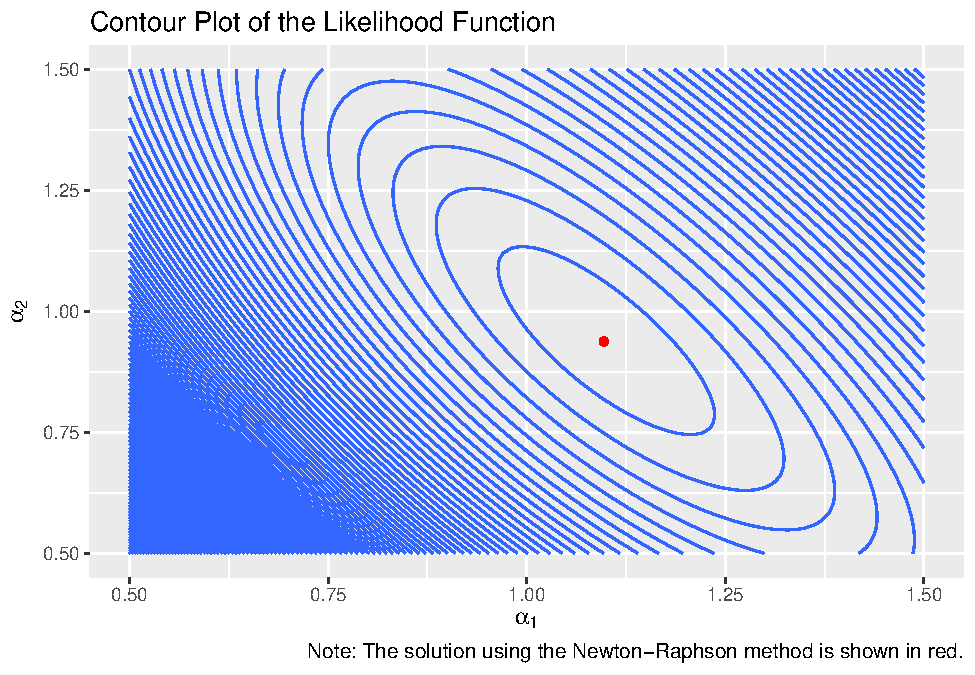
\includegraphics{Atlas-PS_3_files/figure-latex/unnamed-chunk-2-1.pdf}

Next, we implement the Fisher Scoring algorithm.

\begin{Shaded}
\begin{Highlighting}[]
\CommentTok{# We implement the Fisher scoring update method}

\NormalTok{I <-}\StringTok{ }\NormalTok{function(alpha, b, x)\{}
  \KeywordTok{return}\NormalTok{(}\KeywordTok{matrix}\NormalTok{(}\KeywordTok{c}\NormalTok{(}
    \KeywordTok{sum}\NormalTok{(b[, }\DecValTok{1}\NormalTok{]^}\DecValTok{2} \NormalTok{/}\StringTok{ }\NormalTok{(b %*%}\StringTok{ }\NormalTok{alpha)), }
    \KeywordTok{sum}\NormalTok{(}\KeywordTok{apply}\NormalTok{(b, }\DecValTok{1}\NormalTok{, prod) /}\StringTok{ }\NormalTok{(b %*%}\StringTok{ }\NormalTok{alpha)),}
    \KeywordTok{sum}\NormalTok{(}\KeywordTok{apply}\NormalTok{(b, }\DecValTok{1}\NormalTok{, prod) /}\StringTok{ }\NormalTok{(b %*%}\StringTok{ }\NormalTok{alpha)), }
    \KeywordTok{sum}\NormalTok{(b[, }\DecValTok{2}\NormalTok{]^}\DecValTok{2} \NormalTok{/}\StringTok{ }\NormalTok{(b %*%}\StringTok{ }\NormalTok{alpha))}
  \NormalTok{), }\DataTypeTok{ncol=}\DecValTok{2}\NormalTok{))}
\NormalTok{\}}

\NormalTok{fisher_scoring <-}\StringTok{ }\NormalTok{function(I, fprime, alpha0, b, x, }\DataTypeTok{max_iter=}\DecValTok{10000}\NormalTok{, }\DataTypeTok{tol=}\NormalTok{.}\DecValTok{001}\NormalTok{)\{}
  \NormalTok{alpha_t <-}\StringTok{ }\NormalTok{alpha0}
  
  \CommentTok{# Iterate through }
  \NormalTok{for (n in }\DecValTok{1}\NormalTok{:max_iter)\{}
    \CommentTok{# Set stopping conditions}
    \NormalTok{if(}\KeywordTok{sum}\NormalTok{((alpha0 -}\StringTok{ }\NormalTok{alpha_t)^}\DecValTok{2}\NormalTok{) <}\StringTok{ }\NormalTok{tol &}\StringTok{ }\NormalTok{n >}\StringTok{ }\DecValTok{1}\NormalTok{)\{break\}}
    
    \NormalTok{alpha0 <-}\StringTok{ }\NormalTok{alpha_t}
    
    \CommentTok{# Get the Fisher update}
    \NormalTok{alpha_t <-}\StringTok{ }\NormalTok{alpha0 +}\StringTok{ }\KeywordTok{solve}\NormalTok{(}\KeywordTok{I}\NormalTok{(alpha0, b, x)) %*%}\StringTok{ }\KeywordTok{fprime}\NormalTok{(alpha0, b, x) }
  \NormalTok{\}}
  
  \KeywordTok{return}\NormalTok{(}\KeywordTok{c}\NormalTok{(}\DataTypeTok{alpha_t=}\NormalTok{alpha_t, }\DataTypeTok{n=}\NormalTok{n))}
\NormalTok{\}}

\CommentTok{# We call the function on our dataset}
\NormalTok{alpha0 <-}\StringTok{ }\KeywordTok{c}\NormalTok{(}\DecValTok{1}\NormalTok{, }\DecValTok{1}\NormalTok{)}
\NormalTok{b <-}\StringTok{ }\KeywordTok{as.matrix}\NormalTok{(oil[, }\KeywordTok{c}\NormalTok{(}\StringTok{'importexport'}\NormalTok{, }\StringTok{'domestic'}\NormalTok{)])}
\NormalTok{x <-}\StringTok{ }\KeywordTok{as.matrix}\NormalTok{(oil[, }\KeywordTok{c}\NormalTok{(}\StringTok{'spills'}\NormalTok{)])}

\NormalTok{solution <-}\StringTok{ }\KeywordTok{fisher_scoring}\NormalTok{(}\DataTypeTok{I=}\NormalTok{I, }\DataTypeTok{fprime=}\NormalTok{fprime, }\DataTypeTok{alpha0=}\KeywordTok{c}\NormalTok{(}\DecValTok{1}\NormalTok{, }\DecValTok{1}\NormalTok{), }\DataTypeTok{b=}\NormalTok{b, }\DataTypeTok{x=}\NormalTok{x, }\DataTypeTok{tol=}\NormalTok{.}\DecValTok{00001}\NormalTok{)}
\end{Highlighting}
\end{Shaded}

The solution is given as \(\alpha = [1.097, .938]\), converging in 6
iterations. Below, the contour plot for the likelihood function is
shown, with the green dot labelling the given solution. We see that the
algorithm appears to have converged on the solution. Note that this is
the same solution seen above with Newton's Algorithm. This is as
expected, as the two techniques are quite similar.

\begin{Shaded}
\begin{Highlighting}[]
\CommentTok{# Plot the contours with the solution in red}
\KeywordTok{ggplot}\NormalTok{(results) +}\StringTok{ }
\StringTok{  }\KeywordTok{geom_contour}\NormalTok{(}\KeywordTok{aes}\NormalTok{(}\DataTypeTok{x=}\NormalTok{alpha1, }\DataTypeTok{y=}\NormalTok{alpha2, }\DataTypeTok{z=}\NormalTok{likelihood), }\DataTypeTok{bins=}\NormalTok{n_bin) +}\StringTok{ }
\StringTok{  }\KeywordTok{geom_point}\NormalTok{(}\KeywordTok{aes}\NormalTok{(}\DataTypeTok{x=}\NormalTok{solution[}\DecValTok{1}\NormalTok{], }\DataTypeTok{y=}\NormalTok{solution[}\DecValTok{2}\NormalTok{]), }\DataTypeTok{colour=}\StringTok{"green"}\NormalTok{) +}
\StringTok{  }\KeywordTok{xlab}\NormalTok{(}\KeywordTok{TeX}\NormalTok{(}\StringTok{"$}\CharTok{\textbackslash{}\textbackslash{}}\StringTok{alpha_1$"}\NormalTok{)) +}\StringTok{ }\KeywordTok{ylab}\NormalTok{(}\KeywordTok{TeX}\NormalTok{(}\StringTok{"$}\CharTok{\textbackslash{}\textbackslash{}}\StringTok{alpha_2$"}\NormalTok{)) +}\StringTok{ }
\StringTok{  }\KeywordTok{ggtitle}\NormalTok{(}\StringTok{"Contour Plot of the Likelihood Function"}\NormalTok{) +}
\StringTok{  }\KeywordTok{labs}\NormalTok{(}\DataTypeTok{caption=}\StringTok{"Note: The solution using Fisher Scoring is shown in green."}\NormalTok{)}
\end{Highlighting}
\end{Shaded}

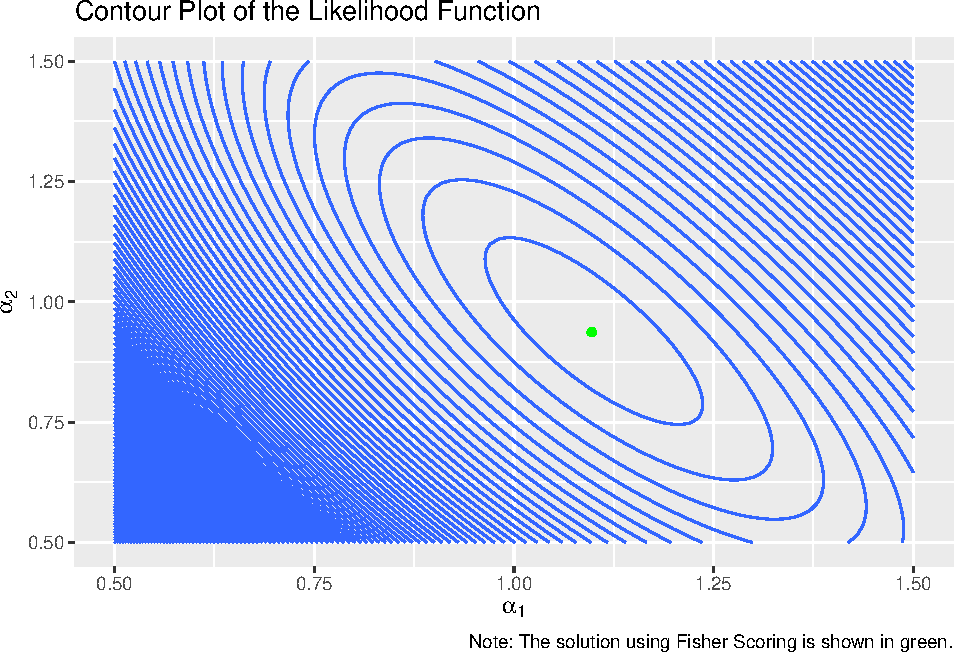
\includegraphics{Atlas-PS_3_files/figure-latex/unnamed-chunk-4-1.pdf}

Both algorithms converge to the same solution, given a starting point
near the correct solution. Fisher scoring takes 2 more iterations to get
there, but roughly comparable. The computation implementation ease is
nearly identical, although because we used the Hessian to get the Fisher
Information, it was an extra step of derivation over Newton's Method. If
the Hessian was more difficult to find, Fisher Scoring would make more
sense.

\subsection{e)}\label{e}

Next, we implement the method of steepest ascent, and apply it to the
problem. We already have the first derivative of the log-likelihood
function above, and so we do not need any further derivation to use the
steepest ascent algorithm with backtracking.

\begin{Shaded}
\begin{Highlighting}[]
\NormalTok{steepest_ascent <-}\StringTok{ }\NormalTok{function(f, fprime, alpha0, b, x, }\DataTypeTok{max_iter=}\DecValTok{10000}\NormalTok{, }\DataTypeTok{tol=}\NormalTok{.}\DecValTok{001}\NormalTok{)\{}
  \NormalTok{alpha_t <-}\StringTok{ }\NormalTok{alpha0}
  \NormalTok{path <-}\StringTok{ }\KeywordTok{matrix}\NormalTok{(}\DataTypeTok{ncol=}\KeywordTok{length}\NormalTok{(alpha0), }\DataTypeTok{nrow=}\DecValTok{0}\NormalTok{)}
  
  \CommentTok{# Iterate through }
  \NormalTok{for (n in }\DecValTok{1}\NormalTok{:max_iter)\{}
    
    \CommentTok{# Set stopping conditions}
    \NormalTok{if(}\KeywordTok{sum}\NormalTok{((alpha0 -}\StringTok{ }\NormalTok{alpha_t)^}\DecValTok{2}\NormalTok{) <}\StringTok{ }\NormalTok{tol &}\StringTok{ }\NormalTok{n >}\StringTok{ }\DecValTok{1}\NormalTok{)\{break\}}
    
    \NormalTok{alpha0 <-}\StringTok{ }\NormalTok{alpha_t}
    
    \CommentTok{# Reset the backtrack scaling to 1}
    \NormalTok{backtrack <-}\StringTok{ }\DecValTok{1} 
    
    \CommentTok{# Get the update h}
    \NormalTok{fprime_x <-}\StringTok{ }\KeywordTok{fprime}\NormalTok{(alpha0, b, x)}
    \NormalTok{M <-}\StringTok{ }\KeywordTok{diag}\NormalTok{(}\KeywordTok{length}\NormalTok{(fprime_x))}
    \NormalTok{h_t <-}\StringTok{ }\NormalTok{backtrack *}\StringTok{ }\NormalTok{(}\KeywordTok{solve}\NormalTok{(M) %*%}\StringTok{ }\NormalTok{fprime_x)}
    
    \CommentTok{# While the next point would be negative, backtrack (divide by 2)}
    \NormalTok{while(}\KeywordTok{f}\NormalTok{(alpha0 +}\StringTok{ }\NormalTok{h_t, b, x) <}\StringTok{ }\KeywordTok{f}\NormalTok{(alpha0, b, x))\{}
      \NormalTok{backtrack <-}\StringTok{ }\NormalTok{backtrack /}\StringTok{ }\DecValTok{2} 
      \NormalTok{h_t <-}\StringTok{ }\NormalTok{backtrack *}\StringTok{ }\NormalTok{(}\KeywordTok{solve}\NormalTok{(M) %*%}\StringTok{ }\NormalTok{fprime_x)}
    \NormalTok{\}}

    \CommentTok{# Iterate to the next point    }
    \NormalTok{alpha_t <-}\StringTok{ }\NormalTok{alpha0 +}\StringTok{ }\NormalTok{h_t}
    \NormalTok{path <-}\StringTok{ }\KeywordTok{rbind}\NormalTok{(path, }\KeywordTok{t}\NormalTok{(alpha0))}
  \NormalTok{\}}
  
  \KeywordTok{return}\NormalTok{(}\KeywordTok{list}\NormalTok{(}\DataTypeTok{path=}\NormalTok{path, }\DataTypeTok{n=}\NormalTok{n, }\DataTypeTok{alpha_t=}\NormalTok{alpha_t))}
\NormalTok{\}}

\NormalTok{solutions <-}\StringTok{ }\KeywordTok{steepest_ascent}\NormalTok{(log_likelihood, fprime, }\KeywordTok{c}\NormalTok{(}\DecValTok{1}\NormalTok{, }\DecValTok{1}\NormalTok{), }\DataTypeTok{b=}\NormalTok{b, }\DataTypeTok{x=}\NormalTok{x, }\DataTypeTok{tol=}\NormalTok{.}\DecValTok{00001}\NormalTok{)}
\end{Highlighting}
\end{Shaded}

The solver works effectively, finding \(\alpha = [1.095, .941]\) in 14
iterations. This is a bit slower than the methods above (Newton's and
Fisher Scoring). However, the derivation here is much easier, as you
only need the first derivative and the likelihood function (no second
derivative or Fisher Information). Below, we plot the solution, and the
path taken to get there.

\begin{Shaded}
\begin{Highlighting}[]
\CommentTok{# Plot the contours with the solution in red}
\KeywordTok{ggplot}\NormalTok{(results) +}\StringTok{ }
\StringTok{  }\KeywordTok{geom_contour}\NormalTok{(}\KeywordTok{aes}\NormalTok{(}\DataTypeTok{x=}\NormalTok{alpha1, }\DataTypeTok{y=}\NormalTok{alpha2, }\DataTypeTok{z=}\NormalTok{likelihood), }\DataTypeTok{bins=}\NormalTok{n_bin) +}\StringTok{ }
\StringTok{  }\KeywordTok{geom_point}\NormalTok{(}\KeywordTok{aes}\NormalTok{(}\DataTypeTok{x=}\NormalTok{solutions$alpha_t[}\DecValTok{1}\NormalTok{], }\DataTypeTok{y=}\NormalTok{solutions$alpha_t[}\DecValTok{2}\NormalTok{]), }\DataTypeTok{colour=}\StringTok{"purple"}\NormalTok{) +}
\StringTok{  }\KeywordTok{geom_path}\NormalTok{(}\DataTypeTok{data=}\KeywordTok{data.frame}\NormalTok{(solutions$path), }\KeywordTok{aes}\NormalTok{(}\DataTypeTok{x=}\NormalTok{X1, }\DataTypeTok{y=}\NormalTok{X2)) +}
\StringTok{  }\KeywordTok{xlab}\NormalTok{(}\KeywordTok{TeX}\NormalTok{(}\StringTok{"$}\CharTok{\textbackslash{}\textbackslash{}}\StringTok{alpha_1$"}\NormalTok{)) +}\StringTok{ }\KeywordTok{ylab}\NormalTok{(}\KeywordTok{TeX}\NormalTok{(}\StringTok{"$}\CharTok{\textbackslash{}\textbackslash{}}\StringTok{alpha_2$"}\NormalTok{)) +}\StringTok{ }
\StringTok{  }\KeywordTok{ggtitle}\NormalTok{(}\StringTok{"Contour Plot of the Likelihood Function"}\NormalTok{) +}
\StringTok{  }\KeywordTok{labs}\NormalTok{(}\DataTypeTok{caption=}\StringTok{"Note: The solution using steepest ascent is shown in purple, with the path taken to get there."}\NormalTok{)}
\end{Highlighting}
\end{Shaded}

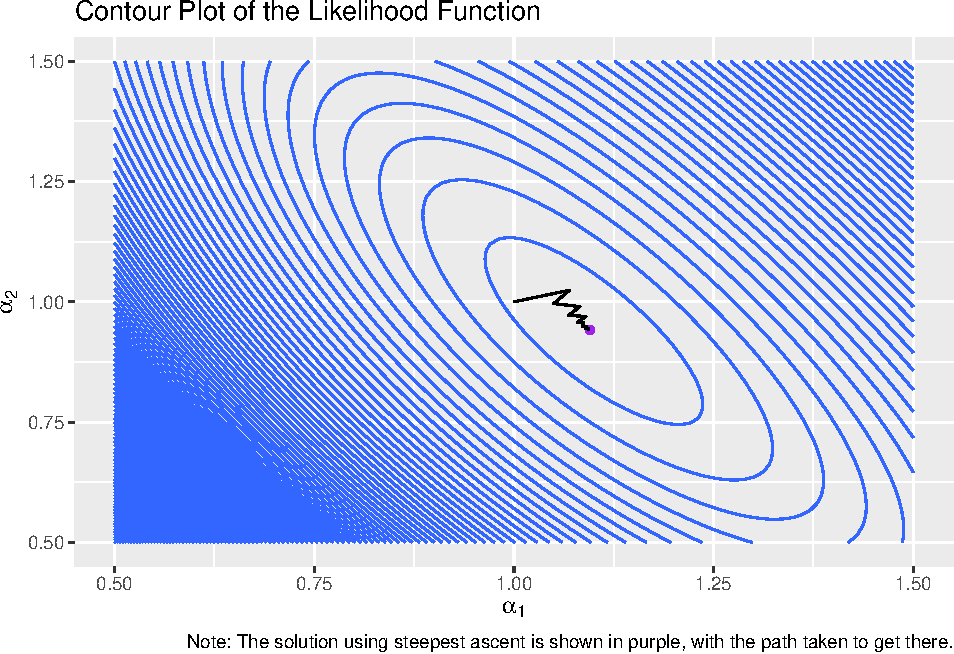
\includegraphics{Atlas-PS_3_files/figure-latex/unnamed-chunk-6-1.pdf}

\section{Problem 2}\label{problem-2}

\subsection{a)}\label{a-1}

Show that the complete-data log-likelihood function is
\(\log{\pi} \summ z_i + \summ z_i \log{\gaus{1}} + \log{(1-\pi)}(n - \summ z_i) + \summ (1 - z_i)\log{\gaus{2}}\)

Given the complete-data density for \(Y\) \[
p(x_i, z_i|\theta) = [\pi \phi(x; \mu_1, \sigma_1^2)]^{z_i}[(1 - \pi)\gaus{2}]^{(1 - z_i)},
\] we can write the complete log-likelihood function for \(\theta\) as
the product of \(n\) random draws from the distribution of \(Y\): \[
L(\theta| x, z)=\prodd[\pi\gaus{1}]^{z_i}[(1 - \pi) \gaus{2}]^{(1 - z_i)}.
\]

We take can then write the log-likelihood

\begin{align*}
l(\theta | x, z) &= \summ \log(\pi \gaus{1})^{z_i} + \summ \log((1-\pi) \gaus{2})^{(1-z_i)} \\
&= \summ z_i \log{\pi} + \summ z_i \log{\gaus{1}} + \summ(1-z_i)\log{(1-\pi)} + \summ(1- z_i) \log{\gaus{2}} \\
&= \log{\pi} \summ z_i + \summ z_i \log{\gaus{1}} + \log{(1-\pi)}(n - \summ z_i) + \summ (1 - z_i)\log{\gaus{2}}
\end{align*}

\subsection{b)}\label{b-1}

Find \(Q(\theta|\theta^{(k)})\).

We then can write \(Q(\theta | \theta^{(k)})\) as the expected value of
the \(l(\theta | Y)\) with respect to the distribution of \(Z\). As
\(X\) is observed, all terms not dependant on \(Z\) are constant. We can
write

\begin{align*}
Q(\theta | \theta^{(k)} &= \rm{E}[\log f_Y(y|\theta) | x, \theta^{(k)}] \\
&= E[\log{\pi} \summ z_i + \summ z_i \log{\gaus{1}} + \log{(1-\pi)}(n - \summ z_i) + \summ (1 - z_i)\log{\gaus{2}}]\\ &= 
\log{\pi} \summ E[Z_i] + \summ E[Z_i] \log{\gaus{1}} + \log{(1-\pi)}(n - \summ E[Z_i]) + \summ (1 - E[Z_i])\log{\gaus{2}}, 
\end{align*}

where \(E[Z_i]\) is conditional on \(x\) and \(\theta^{(k)}\).

\subsection{c)}\label{c-1}

As \(z_i \in {0, 1}, \forall i \in \mathbb{N}\), we can say that

\begin{align*}
E[Z_i | x_i, \theta^{(k)}] &= 0 \times P[Z_i = 0 | x_i, \theta^{(k)}] + 1 \times P[Z_i = 1|x_i, \theta^{(k)}] \\
&= P[Z_i = 1|x_i, \theta^{(k)}].
\end{align*}

Additionally, we can say that

\[P[Z_i = 1|x_i, \theta^{(k)}] = \frac{P(Z_i=1| x_i, \theta^{(k)})}{P(Z_i=1 | x_i, \theta^{(k)}) + P(Z_i=0| x_i, \theta^{(k)})}
\] where
\({P(Z_i=1 | x_i, \theta^{(k)}) + P(Z_i=0| x_i, \theta^{(k)})} = 1\).

Using the given density for \(Y\), and conditioning on
\(\theta=(\pi, \mu_1, \mu_2, \sigma_1^2, \sigma_2^2)\), we can say that

\begin{align*}
P[Z_i = 1 | x_i, \theta^{(k)}] &= [\pi^{(k)}\gausk{1}]^1 [(1- \pi^{(k)})\gausk{2}]^{0} \\ &= \pi^{(k)}\gausk{1}
\end{align*}

and

\begin{align*}
P[Z_i = 0 | x_i, \theta^{(k)}] &= [\pi^{(k)}\gausk{1}]^0 [(1- \pi^{(k)})\gausk{2}]^{1} \\ &=
(1- \pi^{(k)})\gausk{2}
\end{align*}

Combining the two, we can write that \[
E[Z_i | x_i, \theta^{(k)}] = \frac{\pi^{(k)}\gausk{1}}{\pi^{(k)}\gausk{1} + (1- \pi^{(k)})\gausk{2}}
\]

\subsection{d)}\label{d}

To find \(\pi^{(k)}\), we must solve
\(\frac{\partial Q(\theta | \theta^{(k)})}{\partial \pi} = 0\). Using
our equation for \(Q(\theta | \theta^{(k)})\), we can write can write \[
\frac{\partial Q(\theta | \theta^{(k)})}{\partial \pi} = \frac{\summ E[Z_i]}{\pi} - \frac{n - \summ E[Z_i]}{1-\pi}.
\]

Setting the derivative equal to zero and solving for \(\hat{\pi}\) gives
us

\begin{align*}
0 &= \frac{\summ E[Z_i]}{\hat{\pi}} - \frac{n - \summ E[Z_i]}{1-\hat{\pi}} \\
&\implies \hat{\pi}(n - \summ E[Z_i]) = \summ E[Z_i] - \hat{\pi} \summ E[Z_i] \\
&\implies \hat{\pi} n = \summ E[Z_i] \\
&\implies \hat{\pi} = \frac{\summ E[Z_i]}{n} = \frac{\eta^{(k)}}{n}
\end{align*}

\subsection{e)}\label{e-1}

To find the updates for each of the parameters, we take the partial
derivatives for each of the unknown parameters and find their roots. We
use the proportionality given in the assignment.

\subsubsection{\texorpdfstring{Solve for
\(\mu_1^{(k + 1)}\)}{Solve for \textbackslash{}mu\_1\^{}\{(k + 1)\}}}\label{solve-for-mu_1k-1}

\begin{align*}
0 &= \frac{\partial Q(\theta | \theta^{(k)})}{\partial \mu_1} = \summ E[Z_i] \frac{x_i - \hat{\mu1_1}}{\sigma_1^2} \\
&\implies \summ E[Z_i]x_i = \hat{\mu_1} \summ E[Z_i] \\
&\implies \hat{\mu_1} = \frac{\summ E[Z_i] x_i}{\summ E[Z_i]} = \frac{1}{\eta^{(k)}}\summ \eta^{(k)}_i x_i
\end{align*}

\subsubsection{\texorpdfstring{Solve for
\((\sigma_1^2)^{(k + 1)}\)}{Solve for (\textbackslash{}sigma\_1\^{}2)\^{}\{(k + 1)\}}}\label{solve-for-sigma_12k-1}

\begin{align*}
0 &= \frac{\partial Q(\theta | \theta^{(k)})}{\partial \sigma_1^{2}} = \summ E[Z_i] \left(- \frac{1}{2 \sigma_1^2} + 
\frac{(x_i - \mu_1)^2}{ 2 (\sigma_1^2)^2}\right) \\
&\implies 0 = \summ E[Z_i] \left( 
- \frac{1}{2 \hat{\sigma_1^2}} + 
\frac{(x_i - \mu_1)^2}{(2 \hat{\sigma_1^2)}^2}
\right) \\
&\implies  \frac{1}{2\hat{\sigma_1^2}} \summ E[Z_i] = \summ E[Z_i] \frac{(x_i - \mu_1)^2}{2 (\hat{\sigma_1^2})^2} \\
&\implies \hat{\sigma_1^2} \summ E[Z_i] = \summ E[Z_i] (x_i - \mu_1)^2 \\
&\implies \hat{\sigma_1^2} \summ E[Z_i] = \summ E[Z_i] (x_i - \mu_1)^2 \\
&\implies \hat{\sigma_1^2} = \frac{\summ E[Z_i] (x_i - \mu_1)^2}{\summ E[Z_i]} = \frac{1}{\eta^{(k)}} \summ \eta^{(k)}_i (x_i - \mu_1)^2
\end{align*}

\subsubsection{\texorpdfstring{Solve for
\(\mu_2^{(k + 1)}\)}{Solve for \textbackslash{}mu\_2\^{}\{(k + 1)\}}}\label{solve-for-mu_2k-1}

\begin{align*}
0 &= \frac{\partial Q(\theta | \theta^{(k)})}{\partial \mu_2} = \summ (1 - E[Z_i]) \frac{x_i - \hat{\mu_2}}{\sigma_2^2} \\
&\implies \hat{\mu_2} \summ (1 - E[Z_i]) = \summ(1 - E[Z_i])x_i \\ 
&\implies \hat{\mu_2} = \frac{\summ(1- E[Z_i])x_i}{\summ(1- E[Z_i])} \\ 
&= \frac{1}{n - \summ E[Z_i]} \summ(1 - E[Z_i])x_i = \frac{1}{n - \eta^{(k)}} \summ(1 - \eta_i^{(k)})x_i
\end{align*}

\subsubsection{\texorpdfstring{Solve for
\((\sigma_2^2)^{(k + 1)}\)}{Solve for (\textbackslash{}sigma\_2\^{}2)\^{}\{(k + 1)\}}}\label{solve-for-sigma_22k-1}

\begin{align*}
\frac{\partial Q(\theta | \theta^{(k)})}{\partial \sigma_2^{2}} &= \summ(1 - E[Z_i])[-\frac{1}{2 \sigma_2^2} + \frac{(x_i -\mu_2)^2}{2(\sigma_2^2)^2}] \\
&\implies \frac{1}{2\hat{\sigma_2^2}} \summ(1 - E[Z_i]) = \frac{1}{2(\hat{\sigma_2^2})} \summ (1 - E[Z_i])(x_i - \mu_2^{(k)})^2 \\
&\implies \hat{\sigma_2^2} = \frac{\summ (1 - E[Z_i]) (x_i - \mu_2^{(k)})^2}{\summ(1 - E[Z_i])}  \\
&= \frac{1}{n - \eta^{(k)}} \summ (1 - \eta^{(k)}_i)(x_i - \mu_2^{(k)})^2
\end{align*}


\end{document}
